
%!TEX TS-program = xelatex
%!TEX encoding = UTF-8 Unicode
\documentclass[xcolor=svgnames,11pt]{beamer}
%\usepackage{latexsym,amssymb,amsfonts,amsmath}



% -------------------- beamer setup --------------------- %

% for Introduction - Part 1 - ... Orientation
% \useoutertheme[subsection=false, shadow]{miniframes} 

\useinnertheme{default}
\beamertemplatenavigationsymbolsempty



% ----------------------- fonts ------------------------ %

\usefonttheme{serif}
\usepackage{palatino}
\usepackage{eulervm} %additional math 




%\usepackage{xltxtra,fontspec,xunicode}
%\defaultfontfeatures{Scale=MatchLowercase}
%\setromanfont[Numbers=Uppercase]{Intuitive}


% Other Palatino font packages, with math
% see also http://tex.stackexchange.com/questions/89610
% and math_fonts.pdf in Latex docs
% --------------------
% \usepackage{pxfonts}
% \usepackage{mathpazo} % add possibly `sc` and `osf` options
% --------------------



% ---------------------- graphics ----------------------- %

\setbeamercolor*{structure}{fg=black}

\usepackage{graphicx}
\usepackage{transparent} % transparent graphics
\usepackage[abs]{overpic}

\usepackage{textcomp}
\usepackage{subcaption}
\graphicspath{{img/}{../}}


\usepackage{caption}
\usepackage{picture}


% ------------------------ tikz ------------------------- %

\usepackage{tikz}
\usetikzlibrary{positioning}
\usetikzlibrary{arrows,decorations.pathmorphing,backgrounds,positioning,fit,matrix,calc}


% ----------------------- minted ------------------------ %

% \usepackage{minted}

% %\usemintedstyle{friendly}
% %\usemintedstyle{autumn}
% %\usemintedstyle{manni}
% %\usemintedstyle{tango}

% \newminted[mlinepython]{python}{fontsize=\small, linenos,
%                		numbersep=11pt,
%                		gobble=4,
%                		frame=lines,
%                         bgcolor=bg,
%                		framesep=3mm}    



% ----------------------- other ------------------------ %

\usepackage{hyperref}
\usepackage{changepage} % for adjust width
\usepackage{csquotes}



% http://tex.stackexchange.com/questions/84936/
\usepackage{enumitem} % Enumitem-Beamer Incompatibility! See
                                % http://tex.stackexchange.com/a/52299/4912
\newlist{arrowlist}{itemize}{1}
\setlist[arrowlist]{label=$\Rightarrow$}


\usepackage[english]{babel}
\usepackage[latin1]{inputenc}

\usepackage[normalem]{ulem}
\hypersetup{%
  colorlinks=true,% hyperlinks will be coloured
  urlcolor=blue,
}
\makeatletter
\DeclareUrlCommand\ULurl@@{%
  \def\UrlFont{\ttfamily\color{blue}}%
  \def\UrlLeft{\uline\bgroup}%
  \def\UrlRight{\egroup}}
\def\ULurl@#1{\hyper@linkurl{\ULurl@@{#1}}{#1}}
\DeclareRobustCommand*\ULurl{\hyper@normalise\ULurl@}
\makeatother


\newenvironment{mydescription}[1]                                               
  {\begin{list}{}%
   {\renewcommand\makelabel[1]{\textbf{##1}\hfill}%
   \settowidth\labelwidth{\makelabel{#1}}%
   \setlength\leftmargin{\labelwidth}
   \addtolength\leftmargin{\labelsep}}}
  {\end{list}}

% cite source for content in the frame in bottom right corner
% usage: \source{here my source}
\usepackage[absolute,overlay]{textpos}
\setbeamercolor{framesource}{fg=gray}
\setbeamerfont{framesource}{size=\scriptsize}
\newcommand{\source}[1]{\begin{textblock*}{5cm}(7.7cm,8.9cm)
    \begin{beamercolorbox}[ht=0.5cm,right]{framesource}
        \usebeamerfont{framesource}\usebeamercolor[fg]{framesource} {#1}
    \end{beamercolorbox}
\end{textblock*}}

%%%%%%%%%%%%%%%%%%%%%%% stretching %%%%%%%%%%%%%%%%%%%%%%%%%%%%%%%

% from http://tex.stackexchange.com/questions/148365 
% and https://gist.github.com/navarroj/7789910

\let\svpar\par
\let\svitemize\itemize
\let\svenditemize\enditemize
\let\svitem\item
\def\newpar{\def\par{\svpar\vfill}}
\def\newitem{\def\item{\vfill\svitem}}
\let\svcenter\center
\let\svendcenter\endcenter
\let\svcolumn\column
\let\svendcolumn\endcolumn
\newlength\columnskip
\columnskip 0pt
\def\newcolumn{%
  \renewenvironment{column}[2]%
    {\svcolumn{##1}\setlength{\parskip}{\columnskip}##2}%
    {\svendcolumn\vspace{\columnskip}}}

\newcommand\stretchy{\only<2>{%
  \newpar\def\item{\svitem\newitem}%
  \renewenvironment{itemize}{\svitemize}{\svenditemize\newpar\par}%
  \renewenvironment{center}{\svcenter\newpar}{\svendcenter\newpar}%
  \newcolumn
}}

%%%%%%%%%%%%%%%%%%%%%%%%%%%%%%%%%%%%%%%%%%%%%%%%%%%%%%%%%%%%%%%%%%%%


\title {Presentation Title}
%\subtitle{}

\author[Felix Hoffmann]{%
  Felix Hoffmann \vspace{0.25cm} \newline % 
  \small felix11h.dev@gmail.com %
}
\institute[]{}
\date{\today}



%%%%%%%%%%%%%%%%%%%%%%%%%%%%%%%%%%%%%%%%%%%%%%

\begin{document}

\definecolor{bg}{rgb}{0.95,0.95,0.95}
\definecolor{tg}{rgb}{0.35,0.35,0.35}


\begin{frame} 
  \titlepage
\end{frame}

\begin{frame}
  \begin{center} 

    \vspace{5.95cm}

    
\includegraphics[width=2.2cm]{by-nc-sa_eu-eps-converted-to.pdf}

    \vspace{0.25cm}

    \small
    This work is licensed under a
    \href{http://creativecommons.org/licenses/by-nc-sa/4.0/}{Creative
      Commons Attribution-NonCommercial-ShareAlike 4.0 International
      License}.

  \end{center}
\end{frame}


\begin{frame}{Spectrum of Reproducibility}

\begin{flushright}
  \Large\mbox{\textit{... in Computational Research}}
\end{flushright}
\vspace{0.3cm} \normalsize

\begin{figure}


\includegraphics[width=1.0\textwidth]{reproducibility_spectrum_clean.png}
\end{figure}

\large
\begin{columns}[t]
  \begin{column}[t]{0.4\textwidth} 
    \onslide<2->
    \begin{itemize}
      \item[] reproduction from\\ descriptions in\\ research article
    \end{itemize}
    \vspace{0.2cm}

    \onslide<3-> 
    \begin{itemize}
      \item[] \textcolor{white}{-----}\Large\textcolor{red}{\textbf{\emph{Tough!}}}
    \end{itemize}

    \large
   
  \end{column}
  \hfill
  \begin{column}[t]{0.45\textwidth} 
    \onslide<4->
    \begin{itemize}
      \item[] same code,\\ \only<5-8>{same machine, }
        \only<9->{\sout{same machine}, }\textcolor{white}{-----}\\ \only<6-9>{same
          researcher}\only<10->{\sout{same researcher}}
    \end{itemize}
    \vspace{0.2cm}

    \begin{itemize}
      \item[]  \onslide<1->\textcolor{white}{-----} \only<7>{
        \Large\textcolor{Green}{\textbf{\emph{Easy!}}}}
      \only<8->{\Large\textcolor{Green}{\textbf{\emph{\sout{Easy!}}}}}
        \onslide<8->  \textcolor{red}{\textbf{\emph{if only!}}}
    \end{itemize}

  \end{column}
\end{columns}

\vspace{1cm}

\end{frame}




\begin{frame}{The problems...  \onslide<5->{\vspace{-0.94cm} 
      \begin{flushright}
        ... the solution \textcolor{white}{--}
      \end{flushright}}}

  % http://rrcns.readthedocs.org/en/latest/version_control.html
  % http://www.phdcomics.com/comics.php?f=1323

  \large
  \begin{columns}
    \begin{column}{0.4\textwidth}
      \vspace{-1.6cm}
      \begin{itemize}[leftmargin=2pt]
        \itemsep18pt
        \item<1->[] Which version of my code did I use?
        \item<2->[] What parameters?
        \item<3->[] \enquote{It worked yesterday.}
        \item<4->[] \enquote{Why did I do that?}
      \end{itemize}
    \end{column}
    \begin{column}{0.55\textwidth}
      \onslide<6->
      \vspace{-1.cm}
      \begin{center}
        \textbf{\textit{laboratory notebook}}
      \end{center}
      \vspace{-0.95cm}
      \begin{figure}
        \centering

        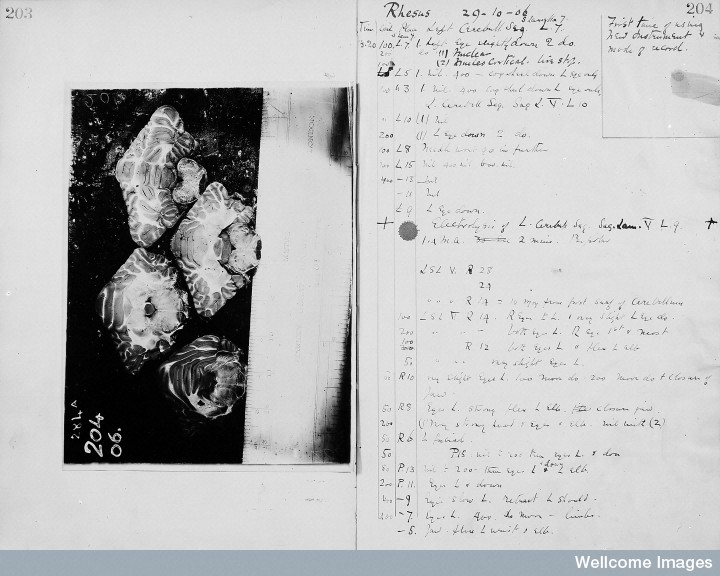
\includegraphics{victor_horsely.jpg}
        % http://wellcomeimages.org/indexplus/image/M0016267.html
        \vspace{-0.28cm}
        \caption*{\tiny \textcopyright Wellcome Library, London 
             \href{http://creativecommons.org/licenses/by/4.0/}{CC BY
               4.0}}
      \end{figure}

      \onslide<7->
      \vspace{-0.72cm}
      \begin{center}
        \textit{... in traditional, experiment-based research}.
      \end{center}
    \end{column}

  \end{columns}

\end{frame}


\begin{frame}{
\includegraphics[width=2.0cm]{sumatra_logo_up.png}
     \textcolor{white}{-}- \textcolor{white}{-}Simulation Management
     Tool}

   \large
   \vspace{0.3cm}
   \onslide<2->
   \begin{center}
     \enquote{\textit{An automated lab notebook for\\ computational projects}}
   \end{center}

   \vspace{-0.15cm}
   \begin{center}
     % \only<3>{
     %   \begin{overpic}[width=9cm]{%
     %       sumatra_record_flowchart.png}     
     %   \end{overpic}}
     \only<3>{
     \begin{overpic}[width=9cm]{%
         sumatra_record_flowchart.png}    
     \end{overpic}}
   \end{center}

   \vspace{0.2cm}
   \begin{columns}
     \begin{column}{0.58\textwidth}
       \onslide<4->
       \begin{arrowlist}
         \itemsep14pt
         \item<4-> assumes that code is under version control
         \item<5-> capture information about computation
         \item<6-> make the information accessible through a command line
           and web interface
       \end{arrowlist}
       \vspace{1cm}

     \end{column}
     \begin{column}{0.42\textwidth}
       \only<4>{
         \vspace{-1.7cm}
       \begin{center}
         \begin{figure}
           
\includegraphics[width=2.6cm]{git_logo.png}
           \caption*{\tiny \textcopyright Jason Long
             \href{http://creativecommons.org/licenses/by/3.0/}{CC BY
               3.0}}
         \end{figure}
       \vspace{0.3cm}
       \vfill
       
\includegraphics[width=2.2cm]{mercurial_logo.png}
       \end{center}
       % git logo CC BY 3.0 Jason Long http://git-scm.com/downloads/logos
       % mercurial free software
       }
       
       \only<5>{
         \vspace{-2.15cm}
         \begin{center}
           \texttt{\textbf{\huge smt run}}
         \end{center}
         }

       \only<6>{ 
       \vspace{-1.4cm}
       \begin{center}
         \begin{figure}
           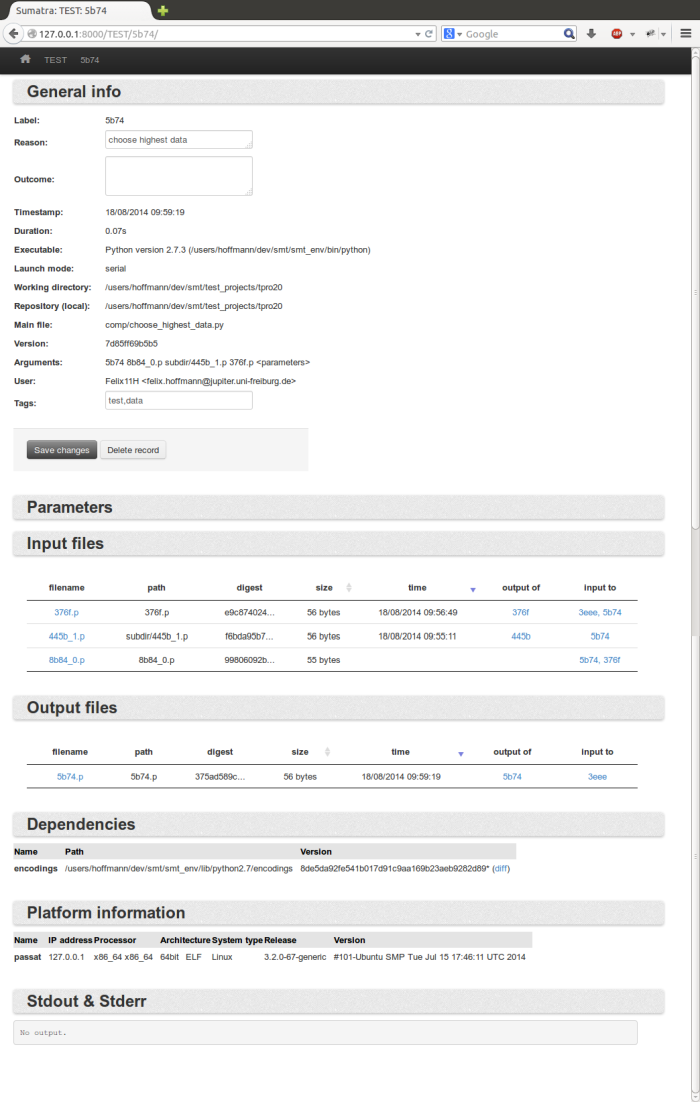
\includegraphics[width=4.2cm]{record_detail.png}
         \end{figure}
       \end{center}
       }
     \end{column}
   \end{columns}

   \vspace{7cm}
  




\end{frame}

\begin{frame}{
\includegraphics[width=2.0cm]{sumatra_logo_up.png}
     \textcolor{white}{-} -\textcolor{white}{-} a tool for
     Reproducible Research}
    
   \large
   \begin{columns}
     \begin{column}{0.58\textwidth}
       By capturing
       \vspace{0.3cm}
       \begin{itemize}
         \itemsep12pt
         \item<2->[] - version of the code
         \item<3->[] - input data
         \item<4->[] - output data
         \item<5->[] - parameters \textcolor{white}{------------} \onslide<6->\makebox(0,0){\put(0,9.2\normalbaselineskip){%
               $\left.\rule{0pt}{4.1\normalbaselineskip}\right\}$ }}
       \end{itemize}

     \end{column}

     \begin{column}{0.42\textwidth}
         \onslide<6->Full replicability of results
     \end{column}
   \end{columns}


        

\end{frame}

\begin{frame}{
\includegraphics[width=2.0cm]{sumatra_logo_up.png}
     \textcolor{white}{-} -\textcolor{white}{-} as an Open Science
     tool}
   \large
   % \begin{center}
   %   computational research project
   % \end{center}

   \begin{tikzpicture}[->,>=stealth',shorten >=1pt,auto,node distance=1.5cm,
     main node/.style={circle, draw}]

		
     \node[draw,rectangle] (crp) at (0,0) {\mbox{computational research project}};
     \onslide<2->
     \node (sc) at (-3.8,-2.25) {scientific code};
     \onslide<3->
     \node (in) at (3.8,-1.7) {input data};
     \onslide<4->
     \node (out) at (3.88,-2.8) {output data};

    


     \onslide<5->
     \node (smt) at (0,-2.25) {
\includegraphics[width=2.0cm]{sumatra_logo.png}};

     \path[every node/.style={font=\sffamily\small, circle,
       draw}, very thick, color=gray]
       (in.west) edge 	[out=180,in=0] ($(smt.east)+(0,0.1)$);
 
     \path[every node/.style={font=\sffamily\small, circle,
       draw}, very thick, color=gray]
       ($(smt.east)+(0,-0.1)$) edge [out=0,in=180] (out.west);

     \path[every node/.style={font=\sffamily\small, circle,
       draw}, very thick, color=gray, <-]
       ($(smt.west)+(0,-0.1)$) edge ($(sc.east)+(0,-0.1)$)
       ($(sc.east)+(0,0.1)$) edge  ($(smt.west)+(0,0.1)$);
       

     \onslide<6->
     \node (figs) at (-3.8, -5)
     {
\includegraphics[width=3.7cm]{GitHub_padded.png}};

     \onslide<6-8>
     \path[every node/.style={font=\sffamily\small, circle,
       draw}, very thick, color=gray]
       (sc.south) edge (figs.north);

     \onslide<7->
     \node (github) at (3.88, -5)
     {
\includegraphics[width=3.7cm]{figshare-main.png}};
     \onslide<7-8>
     \path[every node/.style={font=\sffamily\small, circle,
       draw}, very thick, color=gray]
       (out.south) edge (github.north);

     \onslide<9->
     \path[every node/.style={font=\sffamily\small, circle,
       draw}, very thick, color=gray]
       (smt.south) edge [out=270,in=180] (github.west)
       (smt.south) edge [out=270,in=0] (figs.east);
                        

     % \useasboundingbox (c) rectangle (-2,1.5) --
     % (c) rectangle (1.5,1.5);

     % \path[every node/.style={font=\sffamily\small, circle,
     %   draw}]
     % (a.20) edge [bend left=15] (b.160)
     % (b.-160) edge [bend right=15] (a.-20) 
     % (a) edge [bend right=15] (c)
     % (b.-120) edge [bend left=15] (c.40)
     % (b.-80) edge [bend left=15] (c.0);
  
   \end{tikzpicture}




 % \begin{columns}
 %    \begin{column}
   % github logo = public domain 
   % figshare logo CC BY 3.0  http://creativecommons.org/licenses/by/3.0/
 \end{frame}



% \begin{frame}{Resources}
%   \begin{columns}
%     \begin{column}
%       Sumatra
%       Website: \href{http://www.neuralensemble.org/sumatra/}
%       Maintainer: Andrew Davison
      
%       Publication:
%     \end{column}

%     \begin{column}{0.5\textwidth}
%       About the presenter:
%         Felix Hoffmann
%         Website: \href{http://felix11h.github.io/}        
%     \end{column}
% \end{frame}


%%%%%%%%%%%%%%%%%%%%%%%%%%%%%%%%%%%%%%%%%%%%%%

% \input{section1}

% \input{section2}

% \input{section3}

%%%%%%%%%%%%%%%%%%%%%%%%%%%%%%%%%%%%%%%%%%%%%%




\end{document}

